\documentclass[aspectratio=169]{beamer}

% Je kan het lettertype iets vergroten door hierboven optie ``14pt'' toe te
% voegen.

%==============================================================================
% Aanloop
%==============================================================================

%---------- Vormgeving --------------------------------------------------------

\usetheme{hogent}

% Kies hieronder een achtergrondkleur
\usecolortheme{hgwhite} % witte achtergrond, zwarte tekst
%\usecolortheme{hgblack} % zwarte achtergrond, witte tekst

%---------- Packages ----------------------------------------------------------

\usepackage[dutch]{babel}      % Nederlandse taal: splitsingen, enz.

\usepackage{booktabs}          % Mooie tabellen
\usepackage{multirow,multicol} % Tabelcellen samenvoegen
\usepackage{eurosym}           % Euro symbool
\usepackage{amssymb,latexsym,amsfonts,graphicx}

%---------- Commando-definities -----------------------------------------------

\newtheorem{definitie}{Definitie}[]
\newtheorem{eigenschap}{Eigenschap}[]

%---------- Info over de presentatie ------------------------------------------

\title[It Fundamentals]{It Fundamentals}
\subtitle{subtitel}
\author{Jens Buysse, Karine Van Driessche, Koen Mertens, Lieven Smits}
\date{\today}

%==============================================================================
% Inhoud presentatie
%==============================================================================

\begin{document}

%---------- Titelpagina, inhoudstafel -----------------------------------------

\frame{\maketitle}

\begin{frame}[allowframebreaks]
  \frametitle{Inhoud.}

  \tableofcontents
\end{frame}
 
%---------- Corpus ------------------------------------------------------------


	\section{Inleiding}
\frame{\tableofcontents[currentsection]}

\subsection{Het veld $\mathbb{R},+,.$}
\begin{frame}
\frametitle{Eigenschappen in $\mathbb{R},+,.$}
\pause
\begin{eigenschap}
Stel $x,y,z\in \mathbb{R}$
\pause
\begin{itemize}
\item<+-> $\mathbb{R}$ is gesloten voor $+$ en $\cdot$: $x+y \in \mathbb{R}$ en $x\cdot  y \in \mathbb{R}$.
\item<+-> commutatief: $x+y=y+x$ en $x\cdot  y=y \cdot  x$.
\item<+-> associatief: $(x+y)+z=x+(y+z)$ en $(x\cdot  y)\cdot z = x\cdot  (y\cdot z)$.
\item<+-> distributief: $x\cdot (y+z)=x\cdot  y+x\cdot z$.
\item<+-> neutraal element: $x+0=x$ en $x\cdot  1=x$.
\item<+-> invers element voor +: er bestaat een element $-x\in \mathbb{R}$ zodat $x+(-x)=0$.
\item<+-> invers element voor $\cdot$: voor elke $x\in \mathbb{R}_{0}$ bestaat er een element $x^{-1}$ zodat $x\cdot  x^{-1}=1$.
\end{itemize}
\pause
Besluit: $\mathbb{R},+,\cdot $ is een veld.
\end{eigenschap}
\end{frame}

\subsection{Machten}
\begin{frame}
\frametitle{Definitie van een macht}
\pause
\begin{definitie}
Stel $a \in \mathbb{R}_0^+ \setminus \{1\}$
\begin{itemize}
\item<+-> dan geldt voor alle $n \in \mathbb{N}_0$
      \pause
      \[\begin{array}{rcl}
        a^n & = & a\cdot a\cdot a \cdots a ~~~(n\geq 2) \\ \pause
        a^1 & = & a \\ \pause
        a^0 & = & 1 \\ \pause
        a^{-n} & = & \frac{1}{a^n} \\ \pause
        a^{-1} & = & \frac{1}{a} \pause
        \end{array}\]
\item<+-> dan geldt voor alle $p,q \in \mathbb{N}$ \pause
      \[\begin{array}{rcl}
        a^{\frac{p}{q}} & = & \sqrt[q]{a^p} ~~~(q\geq 2)\\ \pause
        a^{-\frac{p}{q}} & = & \frac{1}{a^{\frac{p}{q}}} ~~~(q\geq 2)
        \end{array}\]
\end{itemize}
\end{definitie}
\end{frame}

\begin{frame}
\frametitle{Rekenregels}
\pause
\begin{eigenschap}
Stel $a,b \in \mathbb{R}_0^+\setminus\{1\}$. \\
Voor alle $r,s \in \mathbb{Q}$ geldt 
\pause
\[\begin{array}{rcl}
  a^r\cdot a^s & = & a^{r+s} \\~\\  \pause
  \displaystyle \frac{a^r}{a^s} & = & a^{r-s} \\~\\ \pause
  (a^r)^s & = & a^{rs} \\~\\ \pause
  a^r\cdot b^r & = & (a\cdot b)^r \\~\\ \pause
  \displaystyle\frac{a^r}{b^r} & = & \displaystyle(\frac{a}{b})^r
  \end{array}\]
\end{eigenschap}
\end{frame}

\subsection{Logaritmen}
\begin{frame}
\frametitle{Definitie van een logaritme}
\pause
\begin{definitie}

\end{definitie}
\end{frame}

\begin{frame}
\frametitle{Rekenregels}
\pause
\begin{eigenschap}

\end{eigenschap}
\end{frame}

\subsection{Intervallen in $\mathbb{R}$}
\begin{frame}
\frametitle{Notaties}
\pause
\begin{itemize}
\item<+-> Open interval:
      \[ ]a,b[=\{x\in \mathbb{R} | a<x<b\} \subseteq \mathbb{R} \]
\item<+-> Gesloten interval:
      \[ [a,b]=\{x\in \mathbb{R} | a\leq x \leq b\} \subseteq \mathbb{R} \]
\item<+-> Halfopen interval:
      \[ \begin{array}{l}
         [a,b[=\{x\in \mathbb{R} | a \leq x<b\} \subseteq \mathbb{R} \\
         ]a,b]=\{x\in \mathbb{R} | a < x \leq b\} \subseteq \mathbb{R} 
         \end{array}\]
\item<+-> De verzameling van de re\"ele getallen ($\mathbb{R}$):
      \[ \mathbb{R} = ]-\infty,+\infty[ \]
\end{itemize}
\end{frame}


\subsection{Het begrip oneindig in de wiskunde}
\begin{frame}
\frametitle{De uitgebreide re\"ele rechte}
\pause
\begin{definitie}
De {\bf uitgebreide re\"ele rechte} $\overline{\mathbb{R}}$ is:\\~\\
\[ \overline{\mathbb{R}} = \mathbb{R} \cup  \{-\infty,+\infty\} = [-\infty,+\infty] \]~\\
met $-\infty < x < +\infty$ voor elke $x \in \mathbb{R}$.
\end{definitie}
\end{frame}

\begin{frame}
\frametitle{Rekenregels voor `+' en `-' in $\overline{\mathbb{R}}$}
\pause
\begin{eigenschap}
Voor elke $x \in \mathbb{R}$ geldt \pause
\[\begin{array}{rcl}
  +\infty + x & = & +\infty\\ \pause
  -\infty + x & = & -\infty\\ \pause
  +\infty + (+\infty) & = & +\infty\\ \pause
  -\infty + (-\infty) & = & -\infty \pause
  \end{array} \]
\end{eigenschap}
~\\
\pause
Let op! De volgende bewerkingen zijn niet gedefinieerd
\pause
\[\begin{array}{c}
  +\infty + (-\infty) \\ \pause
  -\infty + (+\infty) 
  \end{array} \]
\end{frame}

\begin{frame}
\frametitle{Rekenregels voor `$\times$' en `$/$' in $\overline{\mathbb{R}}$}
\pause
\begin{eigenschap}
Voor elke $x \in \mathbb{R}_0^+$ geldt \pause
\[\begin{array}{rcl}
  +\infty \cdot  x & = & +\infty\\ \pause
  -\infty \cdot  x & = & -\infty\\ \pause
  +\infty / x & = & +\infty\\ \pause
  -\infty / x & = & -\infty   \pause
  \end{array} \]
\end{eigenschap}
\end{frame}

\begin{frame}
\frametitle{Rekenregels voor `$\times$' en `$/$' in $\overline{\mathbb{R}}$}
\begin{eigenschap}
Voor elke $x \in \mathbb{R}_0^-$ geldt \pause
\[\begin{array}{rcl}
  +\infty \cdot  x & = & -\infty\\ \pause
  -\infty \cdot  x & = & +\infty\\ \pause
  +\infty / x & = & -\infty\\ \pause
  -\infty / x & = & +\infty  \pause
  \end{array} \] 
\end{eigenschap}
\end{frame}

\begin{frame}
\frametitle{Rekenregels voor `$\times$' en `$/$' in $\overline{\mathbb{R}}$}
\begin{eigenschap}
Voor elke $x \in \mathbb{R}$ geldt \pause
\[\begin{array}{rcl}
  x/+\infty  & = & 0\\ \pause
  x/-\infty  & = & 0   
  \end{array} \]  
 \end{eigenschap}
\end{frame}

\begin{frame}
\frametitle{Rekenregels voor `$\times$' en `$/$' in $\overline{\mathbb{R}}$}
\begin{eigenschap}
Er geldt \pause
\[\begin{array}{rcl}
  +\infty \cdot  (+\infty) & = & +\infty\\ \pause
  -\infty \cdot  (-\infty) & = & +\infty\\ \pause
  +\infty \cdot  (-\infty) & = & -\infty\\ \pause
  -\infty \cdot  (+\infty) & = & -\infty  \pause
  \end{array} \]
\end{eigenschap}
 \pause
Let op! De volgende bewerkingen zijn niet gedefinieerd
\pause
\[\begin{array}{l}
  0\cdot  (+\infty)\\ \pause
  0\cdot  (-\infty)\\  \pause
  \infty / \infty \\ \pause
  0 / 0 \\  \pause
  0^0\\ \pause
  \infty^0  
  \end{array} \]
 \end{frame}
 
 
	\section{Begrippen}
\frame{\tableofcontents[currentsection]}

\subsection{Definities en notaties}

\begin{frame}
\frametitle{Een re\"ele functie}
\pause
\begin{definitie} 
Een functie $f$ is een {\bfseries re\"ele functie} indien zijn bron- en doelverzameling beide $\mathbb{R}$ zijn. D.w.z.\ dat voor elke $x \in \mathbb{R}$ hoogstens \'e\'en $ y \in \mathbb{R}$ bestaat zodanig dat $f(x) =y $.\\
We noemen $x$ het {\bfseries argument} terwijl $y$ het {\bfseries beeld} wordt genoemd.
\end{definitie}
~\\
\pause
{\bfseries Notaties} ~\\
$f : \mathbb{R} \rightarrow \mathbb{R} : x \mapsto y$\\
${\mathcal{F}}(\mathbb{R},\mathbb{R}) =$ de verzameling van alle re\"ele functies.
\end{frame}

\begin{frame}
\frametitle{Het domein van een functie} 
\pause
\begin{definitie} 
Beschouw de functie $f:X\rightarrow Y:x\mapsto y=f(x)$.\\~
\pause

Het {\bfseries domein} of {\bfseries definitiegebied} van de functie $f$ is de verzameling van alle elementen $x\in X$ waarvoor $f(x) \in Y$:
\[\mbox{dom\,} f = \{x \in X \,|\, \mbox{er bestaat een } y \in Y \mbox{ zodat } y=f(x)\}.\]
\end{definitie}
\end{frame}

\begin{frame}
\frametitle{Het beeld van een functie} 
\pause
\begin{definitie}
	Beschouw de functie $f:X\rightarrow Y:x\mapsto y=f(x)$.\\~
	\pause
	
	Het {\bfseries beeld} van de functie $f$ is de verzameling van alle elementen $y$ waarvoor \mbox{$y=f(x)$} met $x \in X$:
	\[\mbox{bld\,} f = \{y \in Y \,|\, \mbox{er bestaat een } x \in X \mbox{ zodat } f(x)=y \}.\]
\end{definitie}
\end{frame}

\begin{frame}
\frametitle{Het begrip continu} 
\pause
\begin{definitie} Een intu\"{\i}tieve definitie:
	\pause
	\begin{itemize}
		\item<+-> Een re\"ele functie $f$ is {\bfseries continu}, indien we de grafiek van $f$ kunnen tekenen zonder ons potlood op te heffen. \\
		\item<+-> Een re\"ele functie $f$ is {\bfseries continu in een punt $a$} van haar domein, indien de grafiek van $f$ geen `sprong' vertoont in de onmiddellijke omgeving van het punt $(a,f(a))$. In het ander geval spreekt men van een {\bfseries discontinu\"{\i}teit in het punt $a$}. 
	\end{itemize}
\end{definitie}
\end{frame}

\begin{frame}
\frametitle{Een nulpunt van een functie $f$}
\pause
\begin{definitie}
Een {\bfseries nulpunt $x$} van een re\"ele functie $f$ is een element van het domein van $f$ waarvoor de functiewaarde gelijk is aan 0.\\ %snijpunt van de functie $f$ met de $X$-as (de rechte met vergelijking $y=0$).
M.a.w.\ een nulpunt $x$ van een functie $f$ is oplossing van de vergelijking $f(x)=0$.
\end{definitie}
\end{frame}

\begin{frame}
\frametitle{Het snijpunt met de $Y$-as van een functie $f$}
\pause
\begin{definitie}

\end{definitie}
\end{frame}

\begin{frame}
\frametitle{De tekentabel van een functie $f$}
\pause
\begin{definitie}
	
\end{definitie}
\end{frame}

\begin{frame}
\frametitle{Een asymptoot van een functie $f$}
\pause
\begin{definitie}
	
\end{definitie}
\end{frame}



	\section{Veeltermfuncties}
\frame{\tableofcontents[currentsection]}

\subsection{Definitie en notatie}


\begin{frame}
\frametitle{Een veeltermfunctie}
\pause
\begin{definitie}
Een {\bfseries veeltermfunctie} is een re\"ele functie met als functievoorschrift
\[f:\mathbb{R}\rightarrow \mathbb{R}:x\mapsto f(x) = a_n x^n+a_{n-1}x^{n-1}+ \cdots + a_1 x + a_0,\]
met $n\in \mathbb{N}$ en $a_i \in \mathbb{R}$ ($i=0\ldots n$), $a_n\neq 0$.\\
We noemen $n$ de {\bfseries graad} van $f(x)$ en $a_nx^n$ de {\bfseries hoogste graadsterm}.
\end{definitie}
\end{frame}


\subsection{Constante functies}
\begin{frame}
\frametitle{Een constante functie}
\pause
\begin{definitie}
Een {\bfseries constante functie} is een functie waarbij de functiewaarde constant is.
\[ f:\mathbb{R} \rightarrow \mathbb{R} :x\mapsto f(x)=a ~~~~~~ (a \in \mathbb{R})\]
\end{definitie}
\end{frame}

\begin{frame}
\frametitle{ De grafiek}
De grafiek van  $f:\mathbb{R}\rightarrow \mathbb{R}:x\mapsto a$ $(a \in \mathbb{R})$ is 
\begin{figure}[htb]
\begin{center}
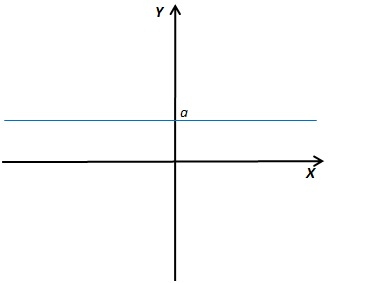
\includegraphics[width=2.7in]{figuren/constantefnct.jpg}
%\caption{De grafiek van de constante functie $y=a$.}\label{constantefnct}
\end{center}
\end{figure}
\end{frame}

\begin{frame}
\frametitle{Eigenschappen}
\pause
\begin{eigenschap}
Voor $f:\mathbb{R}\rightarrow \mathbb{R}:x\mapsto a$ $(a \in \mathbb{R})$ geldt
\begin{itemize}
\item dom$(f)=\mathbb{R}$.
\item bld$(f)=\{a\}$.
\item $f$ is continu in $\mathbb{R}$.
\item De nulpunten zijn:
      \begin{itemize}
      \item als $a\neq 0$ dan zijn er geen nulpunten;
      \item als $a=0$ dan is elke $x\in \mathbb{R}$ een nulpunt van $f$.
      \end{itemize}
\item Het snijpunt met de $Y$-as is:
      $(0,a)$ .
\end{itemize}
\end{eigenschap}
\end{frame}

\begin{frame}
\frametitle{Tekenverloop}
\pause
Voor $f:\mathbb{R}\rightarrow \mathbb{R}:x\mapsto a$ $(a \in \mathbb{R})$ geldt
\\~\\
\[\begin{array}{|c|lcr|}
  \hline
  x&-\infty ~~~~~ & ~~~ & +\infty\\
  \hline
  f(x)& & \mbox{teken van }a &\\
  \hline
  \end{array}\]
\end{frame}

\begin{frame}
\frametitle{Oefening}
De constante functie $f$ bevat het koppel $(2,-3)$. Bepaal deze functie $f$.\\
\end{frame}

\subsection{Lineaire functies}
\begin{frame}
\frametitle{Een functie van de eerste graad}
\pause
\begin{definitie}
De functie $f:\mathbb{R}\rightarrow \mathbb{R}:x\mapsto ax+b$ waarbij $a$ en $b$ gegeven re\"ele getallen zijn en $a\neq 0$, noemt men een {\bfseries functie van de eerste graad} of {\bfseries lineaire functie}.
\end{definitie}
\end{frame}

\begin{frame}
\frametitle{ De grafiek}
De grafiek van de eerstegraadsfunctie $f:x\mapsto ax+b$ is de rechte met  vergelij\-king $y=ax+b$.
\begin{figure}[htb]
\begin{center}
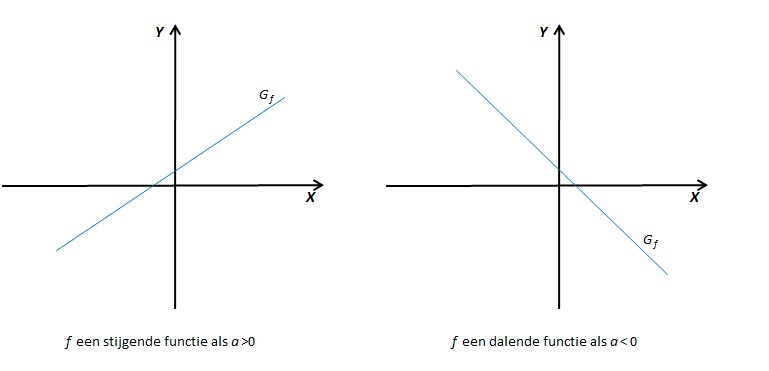
\includegraphics[width=5in]{figuren/rechte.jpg}
\end{center}
\end{figure}
%Het snijpunt met de $X$-as noemen we het {\bfseries nulpunt} van de functie en is de oplos\-sing van de vergelijking $ax+b=0$.

%De co\"effici\"ent $a$ bepaalt de mate waarin de rechte stijgt of daalt en wordt de {\bfseries rich\-tings\-co\"effici\"ent (rico)} van de rechte genoemd.
\end{frame}

\begin{frame}
\frametitle{Eigenschappen}
\pause
\begin{eigenschap}
Voor $f:\mathbb{R}\rightarrow \mathbb{R}:x\mapsto ax+b$ $(a \in \mathbb{R}_0, b\in \mathbb{R})$ geldt
\begin{itemize}
\item dom$(f)=\mathbb{R}$.
\item bld$(f)=\mathbb{R}$.
\item $f$ is continu in $\mathbb{R}$.
\item Het nulpunt is:
      $x={\displaystyle -\frac{b}{a}}$.
\item Het snijpunt met de $Y$-as is:
      $(0,b)$ .
\end{itemize}
\end{eigenschap}
\end{frame}

\begin{frame}
\frametitle{Tekenverloop}
\pause
Voor $f:\mathbb{R}\rightarrow \mathbb{R}:x\mapsto ax+b$ ~~~$(a \in \mathbb{R}_0, b\in \mathbb{R})$ geldt
\\~\\
\[\begin{array}{|c|ccccc|}
  \hline
  x &-\infty& &~~~~~\displaystyle -\frac{b}{a}~~~~~ & &+\infty\\
  \hline
      & &                & &                &\\  
  f(x)& &\mbox{teken van}&0&\mbox{teken van}&\\
      & & -a             & & a &\\
  \hline
  \end{array}\]
\end{frame}

\begin{frame}
\frametitle{Oefeningen}
\pause
\begin{enumerate}
\item[1]<+-> Onderzoek het verloop van de volgende functies van de eerste graad. Teken de grafiek van de functie.
      \begin{enumerate}
      \item[(a)]<+-> $f:x\mapsto x-3$.
      \item[(b)]<+-> $g:x\mapsto -\frac{3}{5}x+7$.
      \end{enumerate}~\\
\item[2]<+-> Bepaal het snijpunt van de grafieken van 
      \begin{enumerate}
      \item[(a)]<+-> $f:x\mapsto -3x-2$ en $g:x\mapsto 5x+6$.
      \item[(b)]<+-> $f:x\mapsto -\frac{2}{3}x+\frac{1}{2}$ en $g:x\mapsto \frac{7}{6}x-\frac{1}{6}$.
      \item[(c)]<+-> $f:x\mapsto x\sqrt{3}+6\sqrt{3}$ en $g:x\mapsto -2x\sqrt{3}$.
      \end{enumerate}
\end{enumerate}
\end{frame}

\begin{frame}
\frametitle{Oefeningen}
\begin{enumerate}
\item[3] (Bron\footnote{Bron: I.\ De Pauw, B.\ Masselis, {\em Wiskunde voor multimedia}, Lannoo Campus, 2009.}) Een object beweegt tijdens een computerspel langs een rechte lijn van het punt $A$ met co\"ordinaten $(0,20)$ naar het punt $B$
met co\"ordinaten $(15,30)$. Zoek de vergelijking van deze rechte. Als het voorwerp in het punt $C$ met co\"ordinaten $(30,40)$ komt, beweegt de speler de joystick, zodat het object $90^\circ$ naar links draait en in een rechte lijn verder beweegt. Vind de vergelijking van de rechte die het nieuwe pad voorstelt. Teken bovendien beide rechten in \'e\'en assenstelsel.\\
Tip: Twee rechten $f$ en $g$, de rechte $f$ met $\mbox{rico} = r_1$ en de rechte $g$ met $\mbox{rico} = r_2$, staan loodrecht op elkaar enkel en alleen als $r_1.r_2=-1$. \\
\end{enumerate}
\end{frame}

\subsection{Functies van de tweede graad}
\begin{frame}
\frametitle{Een functie van de tweede graad}
\pause
\begin{definitie}
Een functie $f:\mathbb{R}\rightarrow \mathbb{R}:x\mapsto ax^2+bx+c$ waarbij $a,b$ en $c$ gegeven re\"ele getallen zijn en waarvoor $a\neq 0$, noemt men een functie van de tweede graad.
\end{definitie}
\end{frame}

\begin{frame}
\frametitle{ De grafiek}
De grafiek van de functie $f:x\mapsto ax^2+bx+c$ is een {\bfseries parabool} $P$.\\
\begin{figure}[htb]
\begin{center}
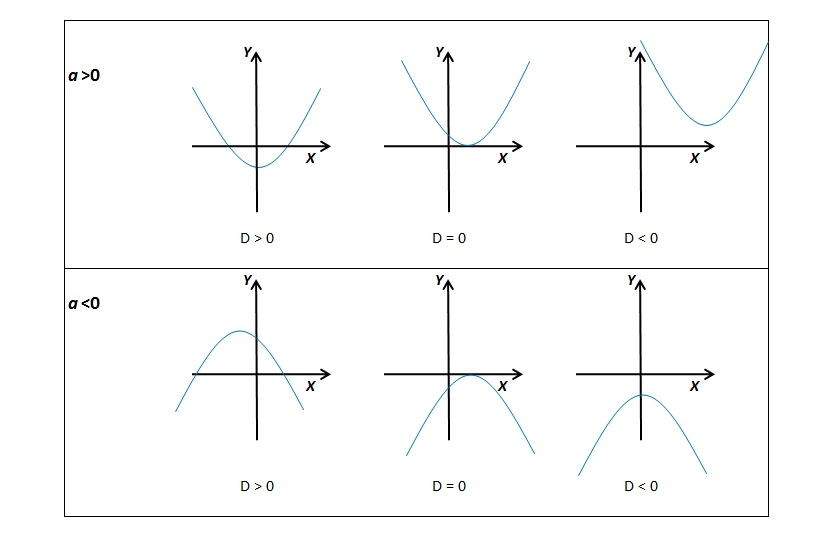
\includegraphics[width=3.5in]{figuren/parabool.jpg}
\end{center}
\end{figure}
met $D=b^2-4ac$
\end{frame}

\begin{frame}
\frametitle{Eigenschappen}
\pause
\begin{eigenschap}
Voor $f:\mathbb{R}\rightarrow \mathbb{R}:x\mapsto ax^2+bx+c$ $(a \in \mathbb{R}_0, b,c\in \mathbb{R})$ geldt
\begin{itemize}
\item dom$(f)=\mathbb{R}$.
\item Het beeld:
      \begin{itemize}
      \item Dalparabool: bld$(f)=[f(-\frac{b}{2a}),+\infty[$.
      \item Bergparabool: bld$(f)=]-\infty,f(-\frac{b}{2a})]$.
      \end{itemize}
\item $f$ is continu in $\mathbb{R}$.
\item Er zijn maximum twee verschillende nulpunten: \\
      $\displaystyle x_{1,2}=\frac{-b\pm \sqrt{D}}{2a}$~~~ met $D=b^2-4ac$.
\item Het snijpunt met de $Y$-as is:
      $(0,c)$ .
\end{itemize}
\end{eigenschap}
\end{frame}

\begin{frame}
\frametitle{Tekenverloop}
\pause
Voor $f:\mathbb{R}\rightarrow \mathbb{R}:x\mapsto ax^2+bx+c$ $(a \in \mathbb{R}_0, b,c\in \mathbb{R})$ geldt
\\~\\
\begin{itemize}
\item $D>0$
      \[\begin{array}{|c|ccccccc|}
        \hline
        x&-\infty& &~x_1~& &~x_2~& &+\infty\\
        \hline
       %     & &                & &                & &                &\\
        f(x)& &\mbox{teken van}&0&\mbox{teken van}&0&\mbox{teken van}&\\
            & & a               && -a            &&a&\\
        \hline
      \end{array}\]
\item $D=0$
      \[\begin{array}{|c|ccccc|}
        \hline
        x&-\infty& &~~~~~~x_1~~~~~~ & &+\infty\\
        \hline
        %    & &                & &                &\\
        f(x)& &~~~\mbox{teken van}~~~&0&~~~\mbox{teken van}~~~&\\
            & & a               & &a&\\
        \hline
      \end{array}\]
\item $D<0$
      \[\begin{array}{|c|ccc|}
        \hline
        x&-\infty&  &+\infty\\
        \hline
        %    & &                & \\
        f(x)& &~~~~~~~~~~~~\mbox{teken van}~~~~~~~~~~~~&\\
            & & a               &\\
        \hline
      \end{array}\]
\end{itemize}\end{frame}

\begin{frame}
\frametitle{Oefeningen}
\pause
\begin{enumerate}
\item<+-> Bespreek de volgende tweedegraadsfuncties:
      \begin{enumerate}
      \item[(a)]<+-> $f:x\mapsto -x^2+2x+5$.
      \item[(b)]<+-> $f:x\mapsto 3x^2+2x+5$.
      \item[(c)]<+-> $f:x\mapsto -x^2+2x-1$.
      \item[(d)]<+-> $f:x\mapsto 3x^2+4x$.
      \item[(e)]<+-> $f:x\mapsto x^2-9$.
      \end{enumerate}
      ~\\
\item<+-> Is de inverse van een tweedegraadsfunctie opnieuw een functie?\\
      Illustreer dit voor de functie $f:x\mapsto f(x)=x^2$.
\end{enumerate}
\end{frame}

\begin{frame}
\frametitle{Extra oefeningen}
\pause
Gegeven
\[\begin{array}{l}
  f:\mathbb{R} \rightarrow \mathbb{R} : x \mapsto f(x)=-2x^2-2x+4\\
	g:\mathbb{R} \rightarrow \mathbb{R} : x \mapsto g(x)=-4x
	\end{array}
\]
Gevraagd:
\begin{enumerate}
\item[a)] Bepaal het domein en beeld van $f$. Geef de nulpunten en het snijpunt met de $Y$-as.\\
      Idem voor de functie $g$.
\item[b)] Teken de grafiek van $f$ en $g$. Duid de snijpunten aan op de grafiek.
\item[c)] Bereken de snijpunten van $f$ en $g$ analytisch.
\item[d)] Geef het functievoorschrift van de volgende functies
      \begin{enumerate}
			\item[i.] $f \circ g$
			\item[ii.] $g \circ f$
			\item[iii.] $g^{-1}$
			\end{enumerate}
\end{enumerate}
\end{frame}

	\section{De exponenti\"ele en logaritmische functie}
\frame{\tableofcontents[currentsection]}

\subsection{De exponenti\"ele functie}
\begin{frame}
\frametitle{De exponenti\"ele functie: defintie} 
\pause
\begin{definitie}
\[f:\mathbb{R} \rightarrow \mathbb{R}:x\mapsto a^x\] 
is de {\bf exponenti\"ele functie met grondtal $a$} $(a\in \mathbb{R}_0^+\setminus \{1\})$.
\end{definitie}
~\\
\pause
\begin{itemize}
\item<+-> Indien $a>1$ is de exponenti\"ele functie strikt stijgend. 
\item<+-> Indien $a<1$ is de exponenti\"ele functie strikt dalend. 
\end{itemize}
\end{frame}

\begin{frame}
\frametitle{Eigenschappen}
\pause
\begin{eigenschap}
Stel $f$ de exponenti\"ele functie met grondtal $a$ $(a\in\mathbb{R}_0^{+}\setminus \{1\})$ :
\pause
\begin{itemize}
\item<+-> $f(0)=1$ 
\item<+-> $f(1)=a$ 
\item<+-> $\mbox{dom}\, f=\mathbb{R}$
\item<+-> $\mbox{bld}\, f=\mathbb{R}_0^+$
\item<+-> De functie $f$ is continu in $\mathbb{R}$.
\item<+-> \pause
      Voor $a>1$ geldt:\\
                 de $X$-as is horizontale asymptoot aan de kant van $-\infty$.\\
          \pause
      Voor $0<a<1$ geldt:\\
                de $X$-as is horizontale asymptoot aan de kant van $+\infty$.
\end{itemize}   
\end{eigenschap}
\end{frame}

\begin{frame}  
\frametitle{De natuurlijke exponenti\"ele functie} 
\pause
\begin{definitie}
De {\bfseries natuurlijke exponenti\"ele functie} met {\bfseries natuurlijk grondtal} e is
\[\mbox{exp}:\mathbb{R} \rightarrow \mathbb{R}:x\mapsto \mbox{exp}(x)=\mbox{e}^x\]
met  ($\mbox{e}=2,7182818284\ldots)$. 
\end{definitie}
\end{frame}

\subsection{De logaritmische functie}
\begin{frame}
\frametitle{De logaritmische functie: definitie} 
\pause
%De inverse functie van de exponenti\"ele functie met grondtal $a$ is de {\bf logaritmi\-sche functie met grondtal $a$}.\\~\\
%\pause
%Dus voor\\
%$f:\mathbb{R} \rightarrow \mathbb{R}:x\mapsto y = a^x$\\
%geldt
%\pause
%\[f^{-1}:\mathbb{R} \rightarrow \mathbb{R}:x\mapsto \mbox{log}_a x\]
%met $y=\mbox{log}_a x \Leftrightarrow x=a^y$\\~\\
%\pause
\begin{definitie} 
De {\bfseries logaritmische functie met grondtal $a$} $(a\in \mathbb{R}_0^+\setminus \{1\})$  is
\[f:\mathbb{R} \rightarrow \mathbb{R}:x\mapsto f(x)=y=\mbox{log}_a x\]
met $a^y=x$.
\end{definitie}
~\\
\pause
\begin{itemize}
\item<+-> Indien $0<a<1$ dan is $\mbox{log}_a$ strikt dalend. 
\item<+-> Indien $a>1$ dan is $\mbox{log}_a$ strikt stijgend. 
\end{itemize}
\end{frame}

\begin{frame}
\frametitle{Eigenschappen}
\pause
\begin{eigenschap}
Stel $f$ de logaritmische functie met grondtal $a$ $(a\in\mathbb{R}_0^{+}\setminus \{1\})$:
 
\pause
\begin{itemize}
\item<+-> $f(1)=0$ 
\item<+-> $f(a)=1$ 
\item<+-> $\mbox{dom}\, f=\mathbb{R}^+_0$
\item<+-> $\mbox{bld}\, f=\mathbb{R}$
\item<+-> De functie $f$ is continu in $\mathbb{R}^+_0$
\item<+-> De $Y$-as is verticale asymptoot
\end{itemize}  
\end{eigenschap} 
\end{frame}

\begin{frame}  
\frametitle{Bijzondere logaritmen} 
\pause
\begin{definitie}~
\begin{itemize}
\item<+-> De {\bfseries Briggse logaritmische functie} is de logaritmische functie met grondtal 10
\[\mbox{log}:\mathbb{R}^+_0 \rightarrow \mathbb{R}: x \mapsto y=\mbox{log}\, x.\]
\item<+-> De {\bfseries Neperiaanse of natuur\-lijke logaritmische} functie is de logaritmische functie met grondtal $e$
\[\mbox{ln}:\mathbb{R}^+_0 \rightarrow \mathbb{R}: x \mapsto y=\mbox{ln}\, x.\]
\item<+-> De logaritmische functie met grondtal $2$ wordt genoteerd als $\mbox{lg}\, x$. 
\[\mbox{lg}:\mathbb{R}^+_0 \rightarrow \mathbb{R}: x \mapsto y=\mbox{lg}\, x.\]
\end{itemize}
\end{definitie}
\end{frame}

\begin{frame}
\frametitle{Voorbeelden}
\pause 
\begin{itemize}
\item<+-> $\mbox{log}_2 16 = \ldots $\\~
\item<+-> $\mbox{log}_3 27 = \ldots $\\~
\item<+-> $\mbox{ln}\, e = \ldots$
\end{itemize}
\end{frame}

\begin{frame}
\frametitle{Rekenregels} 
\pause
\begin{eigenschap}
Stel $a,b \in \mathbb{R}_0^+\setminus\{1\}$.\\~\\
\pause 
\[\begin{array}{rcl}
  \mbox{log}_a(x.y) & = & \mbox{log}_a x + \mbox{log}_a y \\~\\\pause
  \mbox{log}_a\displaystyle \frac{x}{y} & = & \mbox{log}_a x - \mbox{log}_a y \\~\\\pause
  \mbox{log}_a(x^p) & = & p.\mbox{log}_a x  ~~~(\mbox{met } p \in \mathbb{Q})\\ ~\\\pause
  \mbox{log}_a a & = & 1 \\~\\ \pause
  \mbox{log}_a x & = & \frac{\mbox{log}_b x}{\mbox{log}_b a}
  \end{array}\]
\end{eigenschap}~\\
\end{frame}

\begin{frame}
\frametitle{Rekenregels: voorbeelden}
\pause
\begin{itemize}
\item<+-> $\mbox{log} 25 + \mbox{log} 4 = \ldots$\\~
\item<+-> $\mbox{ln} 2\mbox{e}^3 - \mbox{ln} 2 = \ldots$\\~
\item<+-> $4.\mbox{log}_9 3 = \ldots$\\~
\item<+-> $\displaystyle \mbox{lg} 12 = \ldots$
\end{itemize} 
\end{frame}

\subsection*{Oefeningen}

\begin{frame}
\frametitle{Oefeningen}
\pause
\begin{enumerate}
\item<+-> Bepaal het domein en beeld van $f$. Geef de nulpunten, het snijpunt met de $Y$-as en eventuele asymptoten van $f$. Teken ten slotte de grafiek van $f$. 
      \begin{enumerate}
      \item<+->[(a)] $f:\mathbb{R}\rightarrow \mathbb{R}:x\mapsto y=\mbox{log}_3\, x$
      \item<+->[(b)] $f:\mathbb{R}\rightarrow \mathbb{R}:x\mapsto y=2+3^x$
      \item<+->[(c)] $f:\mathbb{R}\rightarrow \mathbb{R}:x\mapsto y=-2\mbox{log}_3\, x$
      \end{enumerate}~\\
\item<+-> Stel 
      \[\begin{array}{c}
        f:\mathbb{R}\rightarrow \mathbb{R}: x\mapsto \mbox{ln(exp}(x))\\
        g:\mathbb{R}\rightarrow \mathbb{R}: x\mapsto \mbox{exp(ln}(x)).
        \end{array}\]
      Wat is het verschil tussen de functie $f$ en de functie $g$?\\
\end{enumerate}
\end{frame}

\begin{frame}
%\frametitle{Oefeningen}
\pause
\small{
\begin{enumerate}
\item<+->[3]
Je speelt het spel Angry Birds. Je moet door boze vogels te lanceren zoveel mogelijk groene varkens raken. Je krijgt hiervoor drie pogingen. Er bevinden zich groene varkens op de punten: $(1,4)$, $(2,4)$, $(2,5)$, $(3,1)$, $(3,3)$, $(3,4)$, $(3,5)$, $(4,2)$, $(4,4)$. \\
Je mag drie vogels lanceren: een bruine, rode en blauwe vogel. 
\begin{itemize}
\item De bruine vogel start in het punt met co\"ordinaten $(1,3)$ en vliegt volgens de grafiek van de functie $f$ met $f(x)= 2^x+1$.
\item De rode vogel start in het punt met co\"ordinaten $(2,0)$ en vliegt volgens de grafiek van de functie $g$ met $g(x)=\lg (x-1)$.
\item De blauwe vogel start in het punt met co\"ordinaten $(2,3)$ en vliegt volgens de grafiek van de functie $h$ met $h(x)=-x^2+6x-5$.
\end{itemize}

Beantwoord de volgende vragen:
\begin{enumerate}
\item[a)] Maak een tekening van de gegeven situatie. Duid eveneens de vlucht van elke vogel op jouw tekening aan. 
%\item[b)] Raakt elke vogel een varken? Zo ja, welk varken wordt er geraakt door welke vogel? \\
%Motiveer jouw antwoord a.d.h.v.\ een analytische berekening. Verifieer vervolgens of jouw berekeningen %overeenstemmen met jouw tekening.
%\item[c)] De varkens met co\"ordinaten $(2,4)$ en $(4,2)$ zijn nog niet geraakt. Je krijgt twee extra vogels om specifiek deze varkens uit te schakelen. Beide vogels vertrekken van het punt met co\"ordinaten $(1,2)$. Ze vliegen allebei volgens een rechte lijn. \\
%Geef voor beide vogels de vergelijking van de functie die hun vlucht volgt.
\end{enumerate}
\end{enumerate}}
\end{frame}

\begin{frame}
%\frametitle{Oefeningen}
%\pause
\small{
\begin{enumerate}
\item<+->[3]
Je speelt het spel Angry Birds. Je moet door boze vogels te lanceren zoveel mogelijk groene varkens raken. Je krijgt hiervoor drie pogingen. Er bevinden zich groene varkens op de punten: $(1,4)$, $(2,4)$, $(2,5)$, $(3,1)$, $(3,3)$, $(3,4)$, $(3,5)$, $(4,2)$, $(4,4)$. \\
Je mag drie vogels lanceren: een bruine, rode en blauwe vogel. 
\begin{itemize}
\item De bruine vogel start in het punt met co\"ordinaten $(1,3)$ en vliegt volgens de grafiek van de functie $f$ met $f(x)= 2^x+1$.
\item De rode vogel start in het punt met co\"ordinaten $(2,0)$ en vliegt volgens de grafiek van de functie $g$ met $g(x)=\lg (x-1)$.
\item De blauwe vogel start in het punt met co\"ordinaten $(2,3)$ en vliegt volgens de grafiek van de functie $h$ met $h(x)=-x^2+6x-5$.
\end{itemize}

Beantwoord de volgende vragen:
\begin{enumerate}
%\item[a)] Maak een tekening van de gegeven situatie. Duid eveneens de vlucht van elke vogel op jouw tekening aan. 
\item[b)] Raakt elke vogel een varken? Zo ja, welk varken wordt er geraakt door welke vogel? \\
Motiveer jouw antwoord a.d.h.v.\ een analytische berekening. Verifieer vervolgens of jouw berekeningen overeenstemmen met jouw tekening.
%\item[c)] De varkens met co\"ordinaten $(2,4)$ en $(4,2)$ zijn nog niet geraakt. Je krijgt twee extra vogels om specifiek deze varkens uit te schakelen. Beide vogels vertrekken van het punt met co\"ordinaten $(1,2)$. Ze vliegen allebei volgens een rechte lijn. \\
%Geef voor beide vogels de vergelijking van de functie die hun vlucht volgt.
\end{enumerate}
\end{enumerate}}
\end{frame}

\begin{frame}
%\frametitle{Oefeningen}
%\pause
\small{
\begin{enumerate}
\item<+->[3]
Je speelt het spel Angry Birds. Je moet door boze vogels te lanceren zoveel mogelijk groene varkens raken. Je krijgt hiervoor drie pogingen. Er bevinden zich groene varkens op de punten: $(1,4)$, $(2,4)$, $(2,5)$, $(3,1)$, $(3,3)$, $(3,4)$, $(3,5)$, $(4,2)$, $(4,4)$. \\
Je mag drie vogels lanceren: een bruine, rode en blauwe vogel. 
\begin{itemize}
\item De bruine vogel start in het punt met co\"ordinaten $(1,3)$ en vliegt volgens de grafiek van de functie $f$ met $f(x)= 2^x+1$.
\item De rode vogel start in het punt met co\"ordinaten $(2,0)$ en vliegt volgens de grafiek van de functie $g$ met $g(x)=\lg (x-1)$.
\item De blauwe vogel start in het punt met co\"ordinaten $(2,3)$ en vliegt volgens de grafiek van de functie $h$ met $h(x)=-x^2+6x-5$.
\end{itemize}

Beantwoord de volgende vragen:
\begin{enumerate}
%\item[a)] Maak een tekening van de gegeven situatie. Duid eveneens de vlucht van elke vogel op jouw tekening aan. 
%\item[b)] Raakt elke vogel een varken? Zo ja, welk varken wordt er geraakt door welke vogel? \\
%Motiveer jouw antwoord a.d.h.v.\ een analytische berekening. Verifieer vervolgens of jouw berekeningen overeenstemmen met jouw tekening.
\item[c)] De varkens met co\"ordinaten $(2,4)$ en $(4,2)$ zijn nog niet geraakt. Je krijgt twee extra vogels om specifiek deze varkens uit te schakelen. Beide vogels vertrekken van het punt met co\"ordinaten $(1,2)$. Ze vliegen allebei volgens een rechte lijn. \\
Geef voor beide vogels de vergelijking van de functie die hun vlucht volgt.
\end{enumerate}
\end{enumerate}}
\end{frame}
	\section{Bijzondere functies}
\frame{\tableofcontents[currentsection]}

\subsection{De absolute waarde functie}
\begin{frame}
\frametitle{Definitie en eigenschappen}
\pause
\begin{definitie}
De {\bf absolute waarde functie} is de functie met als functievoorschrift
\[\mbox{abs}:\mathbb{R}\rightarrow \mathbb{R}:x\mapsto \sqrt{x^2}=\left\{\begin{array}{rr} x& ~~~~~~ \mbox{als } x\geq 0\\-x&\mbox{als } x<0 \end{array}\right.\]
\end{definitie}
%\end{frame}
~\\
%\begin{frame}
%\frametitle{Eigenschappen}
\pause
\begin{eigenschap}
\begin{itemize}
\item<+-> $\mbox{dom(abs)}=\mathbb{R}$
\item<+-> $\mbox{bld(abs)}=\mathbb{R}^{+}$
\item<+-> de functie abs vertoont een knik in het punt $(0,0)$ (cfr.\ singulier punt)
\end{itemize}
\end{eigenschap}
\end{frame}

\subsection{{\em Floor\/} en {\em Ceiling\/} functie}
\begin{frame}
\frametitle{De functie {\em Floor\/}}
\pause
\begin{definitie}
\[\mbox{floor}:\mathbb{R}\rightarrow \mathbb{Z}:x\mapsto \mbox{floor}(x)=z\] 
$\mbox{ met } z \mbox{ het grootste geheel getal zodat } z\leq x$
\end{definitie}
%\end{frame}
~\\
%\begin{frame}
%\frametitle{De functie {\em Floor\/}: eigenschappen}
\pause
\begin{eigenschap}
\pause
\begin{itemize}
\item<+-> $\mbox{dom(floor)}=\mathbb{R}$
\item<+->$\mbox{bld(floor)}=\mathbb{Z}$.
\end{itemize}
\end{eigenschap}
\end{frame}

\begin{frame}
\frametitle{De functie {\em Ceiling\/}}
\pause
\begin{definitie}
\[\mbox{ceiling}:\mathbb{R}\rightarrow \mathbb{Z}:x\mapsto \mbox{ceiling}(x)=z\]
$\mbox{ met } z \mbox{ het kleinste geheel getal zodat } z\geq x$
\end{definitie}
%\end{frame}
~\\
%\begin{frame}
%\frametitle{De functie {\em Ceiling\/}: eigenschappen}
\pause
\begin{eigenschap}
\begin{itemize}
\item<+-> dom(ceiling)$=\mathbb{R}$
\item<+-> bld(ceiling)$=\mathbb{Z}$
\end{itemize}
\end{eigenschap}
\end{frame}

\subsection*{Oefeningen}
\begin{frame}
\frametitle{Oefeningen}
\pause
\begin{enumerate}
\item[1]<+-> Stel $f:\mathbb{R}\rightarrow \mathbb{R}: x\mapsto \mbox{abs}(x+1)$.
      \begin{enumerate}
      \item[(a)] Geef het domein en beeld van $f$.
      \item[(b)] Bepaal alle nulpunten van $f$.
      \item[(c)] Schets de grafiek van $f$.
      \end{enumerate}
      ~\\
      \pause
\item[2]<+-> Stel 
\[\begin{array}{l}
  f:\mathbb{R}\rightarrow \mathbb{R}: x\mapsto \mbox{floor(ceiling}(x-\frac{1}{2}))\\
  g:\mathbb{R}\rightarrow \mathbb{R}: x\mapsto \mbox{floor(ceiling}(x)-\frac{1}{2})\\ 
  h:\mathbb{R}\rightarrow \mathbb{R}: x\mapsto \mbox{ceiling(floor}(x+\frac{1}{2})). 
	\end{array}\]
 Geef voor elk van de gegeven functies het domein en het beeld. Bepaal voor elke functie de nulpunten.
 Teken de grafiek van de functies $f$, $g$ en $h$.
\end{enumerate}
\end{frame}




\end{document}
